\documentclass[12pt]{article}
\usepackage[utf8]{inputenc}
\usepackage{hyperref}
\usepackage{graphicx}
\usepackage[export]{adjustbox}
\usepackage{caption}
\usepackage{subcaption}
\usepackage{fancyhdr}
\usepackage{geometry}
\usepackage{url}
\usepackage{emoji}
\usepackage{float}
\fancyhf{}
\hypersetup{
    colorlinks=true,
    linkcolor=blue,
    filecolor=magenta,      
    urlcolor=cyan,
    pdftitle={designPatterns},
    pdfpagemode=FullScreen,
    }
    
\newcommand\invisiblesection[1]{%
  \refstepcounter{section}%
  \addcontentsline{toc}{section}{\protect\numberline{\thesection}#1}%
  \sectionmark{#1}}
  
    \begin{document}
   
\begin{titlepage}
\invisiblesection{Title Page}
\thispagestyle{empty}
			
	\begin{center}
    
\includegraphics[width=6cm]{UTM-logo.png}
    \end{center}
	
	\begin{center}
	\vspace{0.8cm}
	\LARGE
	University of Toronto Mississauga 
	
	\vspace{0.8cm}
	
	\LARGE
	
	CSC207 Fall 2022
	\vspace{1.7cm}	
	\Large
	
	\textbf{Design Document}
	\vspace{1cm}
	\normalsize	
	
	AUTHORS \\
	\vspace{.3cm}
	\large
	\textbf{Author 1\\ Author 2 \\ Author 3\\ Author 4}

	\normalsize	
	\vspace{1cm}
	GITHUB TEAM: \textbf{team name} \\
	\vspace{.1cm}
        GITHUB URL: \textbf{url} \\
	\begin{center}
	
\includegraphics[height = 2cm]{github.png}
	\end{center}
	\vspace{0.5cm}	
	Month Day Year
	\end{center}
	\newpage
\end{titlepage}

\tableofcontents
    \cfoot{\thepage}
\newpage

\section{Project Identification}
This section should include a concise statement that address such questions as:
\begin{enumerate}
    \item Why are you doing this project (i.e. what is the motivation?)
    \item How will it enhance or add to functionality that already exists (if you are building off a code base)?
\end{enumerate}

\section{User Stories}

User Stories help translate your users’ needs into requirements. To create a list of user stories, start by considering your users’ needs. Each user story will translate to a development task that will be owned by a member of your development team. As you write your user stories, keep in mind you that the user who owns the story will need to create not only an implementation that satisfies the story but also the associated tests.\\
\\
Some examples of user stories are below.
    \begin{center}
      \begin{tabular}{|p{2cm}|p{0.5cm}|p{1.5cm}|p{3cm}|p{3.5cm}|p{1.75cm}|p{1.25cm}|}
        \hline
        \textbf{Name}&\textbf{ID} &\textbf{Owner}&\textbf{Description}&\textbf{Implementation Details}&\textbf{Priority}&\textbf{Effort}
        \\\hline    
        Save File	
        &1.1
        &Jane
        &As a user, I want a UI that allows me to save my progress so that I can continue where I left off when I return to use the software	
        &Create a UI so that users can save progress in whatever folder they would like to on their hard drive.
        &1
        &2
        \\\hline    
        Undo/Redo	
        &1.2
        &Fred
        &As a user, I want options to undo and redo my moves so that I can fix mistakes easily if and when I make them
        &Create an Iterable data structure to store historical moves and actions so these can be easily undone
        &1
        &1      
        \\\hline           
      \end{tabular}
    \end{center}
\noindent Note that you may also want include some user stories that refactor existing code in order to make it more efficient or usable in some way. To include refactoring items in your list, you can use the following syntax:
\begin{center}
\textit{“As a developer, I want … so that …. "} 
\end{center}
An example might be:
\begin{center}
\textit{“As a developer, I want to change the process by which my Tree Objects are indexed so that the application will load 2-3 times more quickly.“} 
\end{center}
Note also that you may include as many user stories as you like.  We will expect you to complete all of those that you mark as high priority (i.e. with a number 1) and we expect each team member to have a suitable amount of work to complete (10-15 hours worth).  But if stories with lower priorities remain once the term is complete, that’s ok; you can always continue to iterate on your product as long as it interests you.
\newpage
\section{Software Design}

This section should describe the design patterns you will use to realize your user stories.  For each design pattern, provide a draft of UML diagrams to show how you’ll implement the pattern as well as a written description that details how it will be used in the context of your user stories.  An example of a pattern description is provided below.  Note that you can adjust these patterns as you progress with your implementation, as this is necessary.
\subsection{Design Pattern 1: Command Pattern}

\noindent \textbf{Overview:} This pattern will be used to implement User Story 1.2 (Undo/Redo).\\

\noindent \textbf{UML Diagram}: Refer to Figure 1, below.\\

\begin{figure}[H]
\begin{center}
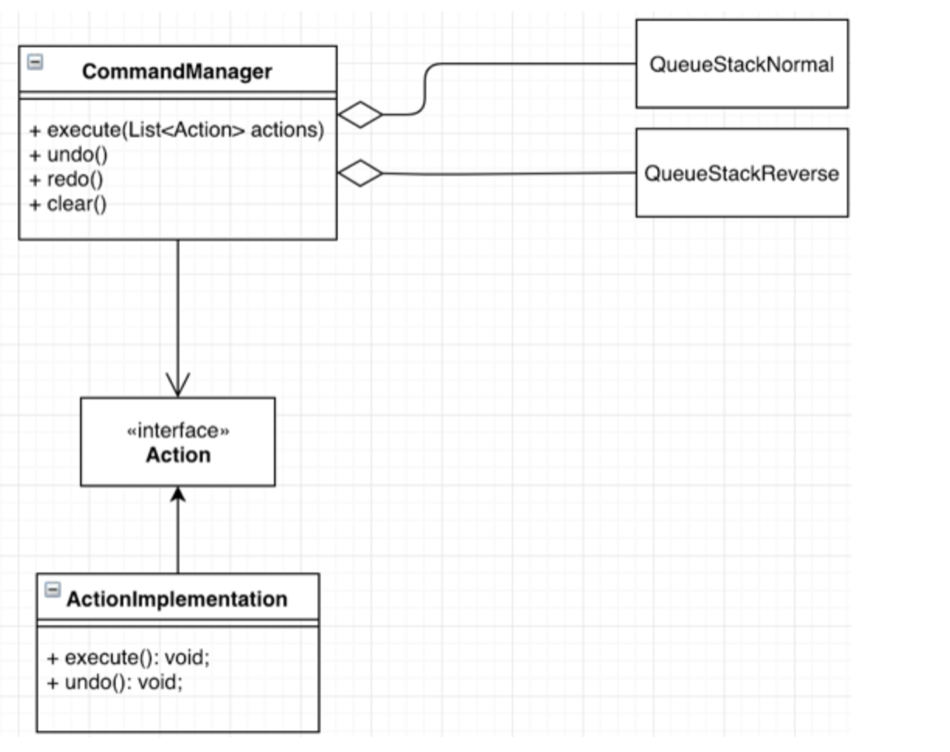
\includegraphics[width=.75\textwidth]{pattern.png}
\end{center}
\caption{The Command Pattern}}
\label{fig:search-space1}
\end{figure}

\newpage
\noindent \textbf{Implementation Details:} The UML diagram outlines these main components:\\
\begin{enumerate}
    \item The Action interface, which includes two methods: execute and undo.
    \item Two modified linked lists (‘QueueStacks’). These will push like a stack and pop like a queue.
    \item The CommandManager, which will execute actions and perform undo/redo.
\end{enumerate}	
The execute method of the CommandManager requires an array of software actions, which are Objects. Every executed action will be registered in the QueueStackNormal.  When performing undo, the action will be popped from this data structure, the undo method will be called and then the action will be pushed to QueueStackReverse.  The opposite will happen when executing the redo operation. The clear method will be used to clear all registered actions in any of the QueueStacks.

\subsection{Design Pattern 2: ?}

\subsection{Design Pattern 3: ?}

\subsection{Design Pattern 4: ?}
\newpage
\section{Expected Timeline}
This section should address such questions as:
\begin{enumerate}
    \item What is the current team’s assessment of the project timeline? 
    \item What are the major milestones?
\end{enumerate}

\noindent The most common tool for project planning in industry is the Gantt Chart
Gantt Chart Template: https://asq.org/quality-resources/gantt-chart

\end{document}
